\section{Evaluation}
\label{sec:evaluation}

Our evaluation systematically assesses LLM-generated synthetic spam across three complementary experimental tracks spanning 4,080 training-evaluation units. Following the methodology framework, we present results organized by research questions: Track 1 evaluates synthetic data for classifier training (RQ1), Track 2a establishes baseline detection capabilities against AI-powered spam (RQ2a), and Track 2b investigates hybrid training strategies (RQ2b).

\subsection{Track 1: Synthetic-to-Real Detection}
\label{sec:eval:track1}

% Figure~\ref{fig:track1} presents performance trajectories (Precision, Recall, F1-Score) across all three prompt strategies (original/strong/weak) for both LLM models and both classifiers. Table~\ref{tab:track1_summary_rf} summarizes baseline and 100\% synthetic performance across all experimental configurations, comparing SVM and Random Forest classifiers across both LLM models and all three prompt strategies.

% Figure~\ref{fig:track1} and Table~\ref{tab:track1_summary_rf}

\begin{figure*}[t]
\centering
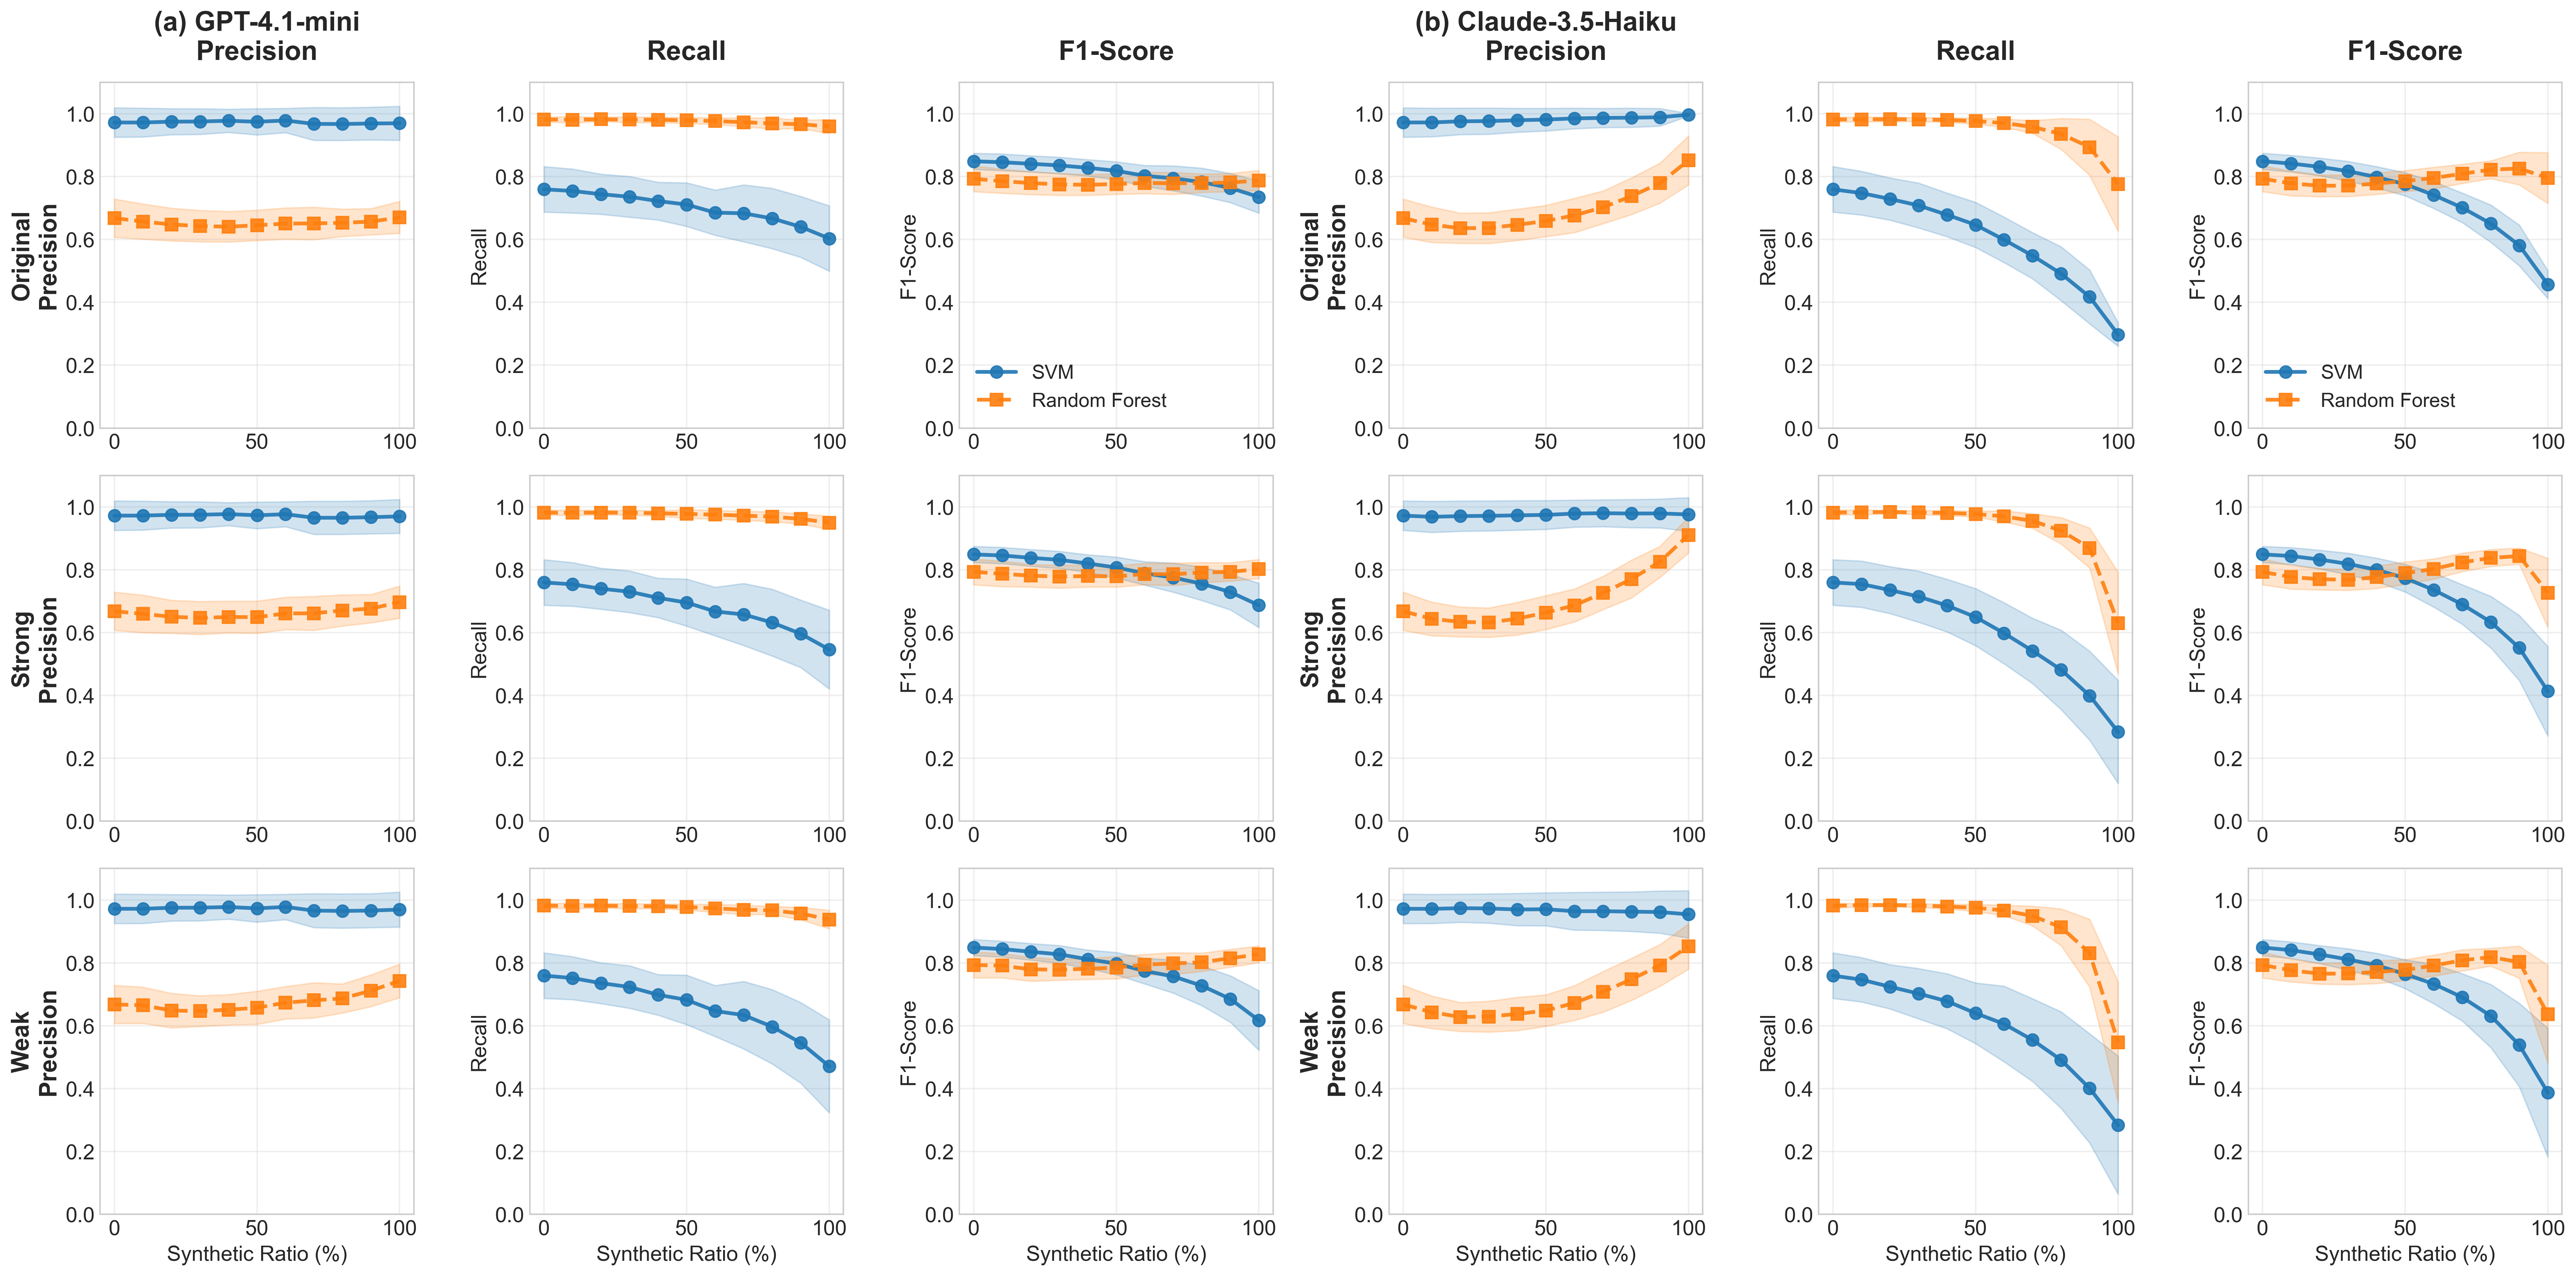
\includegraphics[width=\textwidth]{pic/track1_combined_gpt_claude.png}
\caption{Track 1 - Synthetic-to-Real Detection: Performance metrics (Precision, Recall, F1-Score) across prompt strategies (original/strong/weak, rows) and models (columns). (a) GPT: F1-score exhibits prompt invariance with nearly identical degradation (0.85 $\rightarrow$ 0.70-0.74 at 100\% synthetic, -13.4\% relative). SVM maintains high precision but suffers recall loss. (b) Claude: Shows prompt sensitivity with original/strong prompts degrading moderately (F1 $\rightarrow$ 0.45-0.55 at 100\%, -46.2\% relative), while weak prompt exhibits severe degradation (F1 $\rightarrow$ 0.30-0.40). Shaded regions: $\pm$1 SD across 20 groups.}
\label{fig:track1}
\end{figure*}


\begin{table*}[t]
\centering
\caption{Track 1: Synthetic-to-Real Detection Performance - SVM and Random Forest (RF) Comparison}
\label{tab:track1_summary_rf}
\resizebox{\textwidth}{!}{
\begin{tabular}{lllcccccc}
\toprule
\textbf{Model} & \textbf{Classifier} & \textbf{Prompt} & \multicolumn{3}{c}{\textbf{Baseline (0\% Synthetic)}} & \multicolumn{3}{c}{\textbf{100\% Synthetic}} \\
\cmidrule(lr){4-6} \cmidrule(lr){7-9}
& & & \textbf{Precision} & \textbf{Recall} & \textbf{F1} & \textbf{Precision} & \textbf{Recall} & \textbf{F1} \\
\midrule
\multirow{6}{*}{GPT-4.1-mini}& \multirow{3}{*}{SVM} & Original & \multirow{3}{*}{0.972 $\pm$ 0.047} & \multirow{3}{*}{0.759 $\pm$ 0.072} & \multirow{3}{*}{0.849 $\pm$ 0.026} & 0.970 $\pm$ 0.054 & 0.603 $\pm$ 0.104 & 0.735 $\pm$ 0.051 \\
& & Strong & & & & 0.970 $\pm$ 0.054 & 0.546 $\pm$ 0.125 & 0.687 $\pm$ 0.071 \\
& & Weak & & & & 0.969 $\pm$ 0.056 & 0.471 $\pm$ 0.148 & 0.617 $\pm$ 0.095 \\
& \multirow{3}{*}{Random Forest} & Original & \multirow{3}{*}{0.668 $\pm$ 0.061} & \multirow{3}{*}{0.982 $\pm$ 0.008} & \multirow{3}{*}{0.793 $\pm$ 0.041} & 0.670 $\pm$ 0.051 & 0.959 $\pm$ 0.022 & 0.788 $\pm$ 0.032 \\
& & Strong & & & & 0.697 $\pm$ 0.051 & 0.949 $\pm$ 0.021 & 0.802 $\pm$ 0.030 \\
& & Weak & & & & 0.743 $\pm$ 0.053 & 0.938 $\pm$ 0.029 & 0.827 $\pm$ 0.026 \\
\midrule
\multirow{6}{*}{Claude-3.5-haiku}& \multirow{3}{*}{SVM} & Original & \multirow{3}{*}{0.972 $\pm$ 0.047} & \multirow{3}{*}{0.759 $\pm$ 0.072} & \multirow{3}{*}{0.849 $\pm$ 0.026} & 0.997 $\pm$ 0.004 & 0.297 $\pm$ 0.037 & 0.457 $\pm$ 0.045 \\
& & Strong & & & & 0.976 $\pm$ 0.054 & 0.284 $\pm$ 0.164 & 0.414 $\pm$ 0.142 \\
& & Weak & & & & 0.954 $\pm$ 0.075 & 0.284 $\pm$ 0.220 & 0.387 $\pm$ 0.205 \\
& \multirow{3}{*}{Random Forest} & Original & \multirow{3}{*}{0.668 $\pm$ 0.061} & \multirow{3}{*}{0.982 $\pm$ 0.008} & \multirow{3}{*}{0.793 $\pm$ 0.041} & 0.852 $\pm$ 0.078 & 0.776 $\pm$ 0.150 & 0.796 $\pm$ 0.081 \\
& & Strong & & & & 0.911 $\pm$ 0.057 & 0.630 $\pm$ 0.162 & 0.727 $\pm$ 0.110 \\
& & Weak & & & & 0.852 $\pm$ 0.072 & 0.547 $\pm$ 0.192 & 0.637 $\pm$ 0.156 \\
\bottomrule
\end{tabular}
}
\end{table*}


Performance degradation follows highly linear patterns as synthetic proportion increases, with regression analysis yielding $R^2 > 0.95$ for SVM configurations (detailed in Appendix~\ref{sec:appendix}). This linearity enables reliable interpolation for intermediate mixing ratios and predictable performance boundaries for operational deployment. Random Forest (RF) exhibits near-zero slopes across most configurations, indicating stable performance regardless of synthetic proportion.

Classifier architecture fundamentally determines robustness to synthetic training data. Random Forest (RF) demonstrates substantially higher resilience compared to SVM across both generation models. For GPT at 100\% synthetic training, RF maintains near-baseline F1 (0.788-0.827 vs baseline 0.793), while SVM degrades significantly (0.617-0.735 vs baseline 0.849). For Claude original prompt, RF achieves F1 = 0.796 compared to SVM's F1 = 0.457, representing a 74\% relative advantage. The ensemble architecture's inherent regularization and feature subsampling mechanisms appear to mitigate distributional shift effects between synthetic and real spam.

Precision-recall trade-offs differ fundamentally between architectures. SVM exhibits extreme asymmetry, maintaining near-perfect precision (0.95-1.00) while recall degrades substantially at high synthetic ratios, resulting in overly conservative classification. RF maintains balanced precision-recall profiles with both metrics remaining stable under synthetic data substitution. This suggests SVM learns overly strict decision boundaries from synthetic spam, while RF's ensemble voting mechanism provides more robust generalization.

Prompt strategy critically determines effectiveness for synthetic training. For SVM, original prompts consistently outperform alternatives across both models, establishing that faithful reproduction without artificial amplification or attenuation produces synthetic spam closest to real spam's feature distribution. RF exhibits non-monotonic behavior with prompt sensitivity varying by model, suggesting ensemble methods respond differently to generation intensity.

GPT generates substantially higher-quality synthetic training data than Claude across all configurations. At 100\% synthetic with original prompts, GPT maintains 86.6\% of baseline performance (SVM: 0.849 $\rightarrow$ 0.735) while Claude retains only 53.8\% (0.849 $\rightarrow$ 0.457). The model-dependent quality gap persists across all prompt strategies and classifiers, indicating fundamental differences in generation capabilities rather than prompt engineering artifacts. The superior performance likely stems from better preservation of real spam's lexical diversity and feature co-occurrence patterns.


\subsection{Track 2a: Real-to-Synthetic Detection}
\label{sec:eval:track2a}

% Figure~\ref{fig:track2a} presents detection performance metrics (Precision, Recall, F1-Score) across both classifiers, all prompt strategies, and varying training data sizes. Table~\ref{tab:track2a_2b_combined} (Track 2a columns) presents detection performance across varying training data sizes (100, 150, 200 real spam samples), testing targets (GPT vs Claude synthetic spam), classifiers (SVM vs Random Forest), and all three prompt strategies.

% Figure~\ref{fig:track2a} and Table~\ref{tab:track2a_2b_combined} (Track 2a columns)

\begin{figure*}[t]
\centering
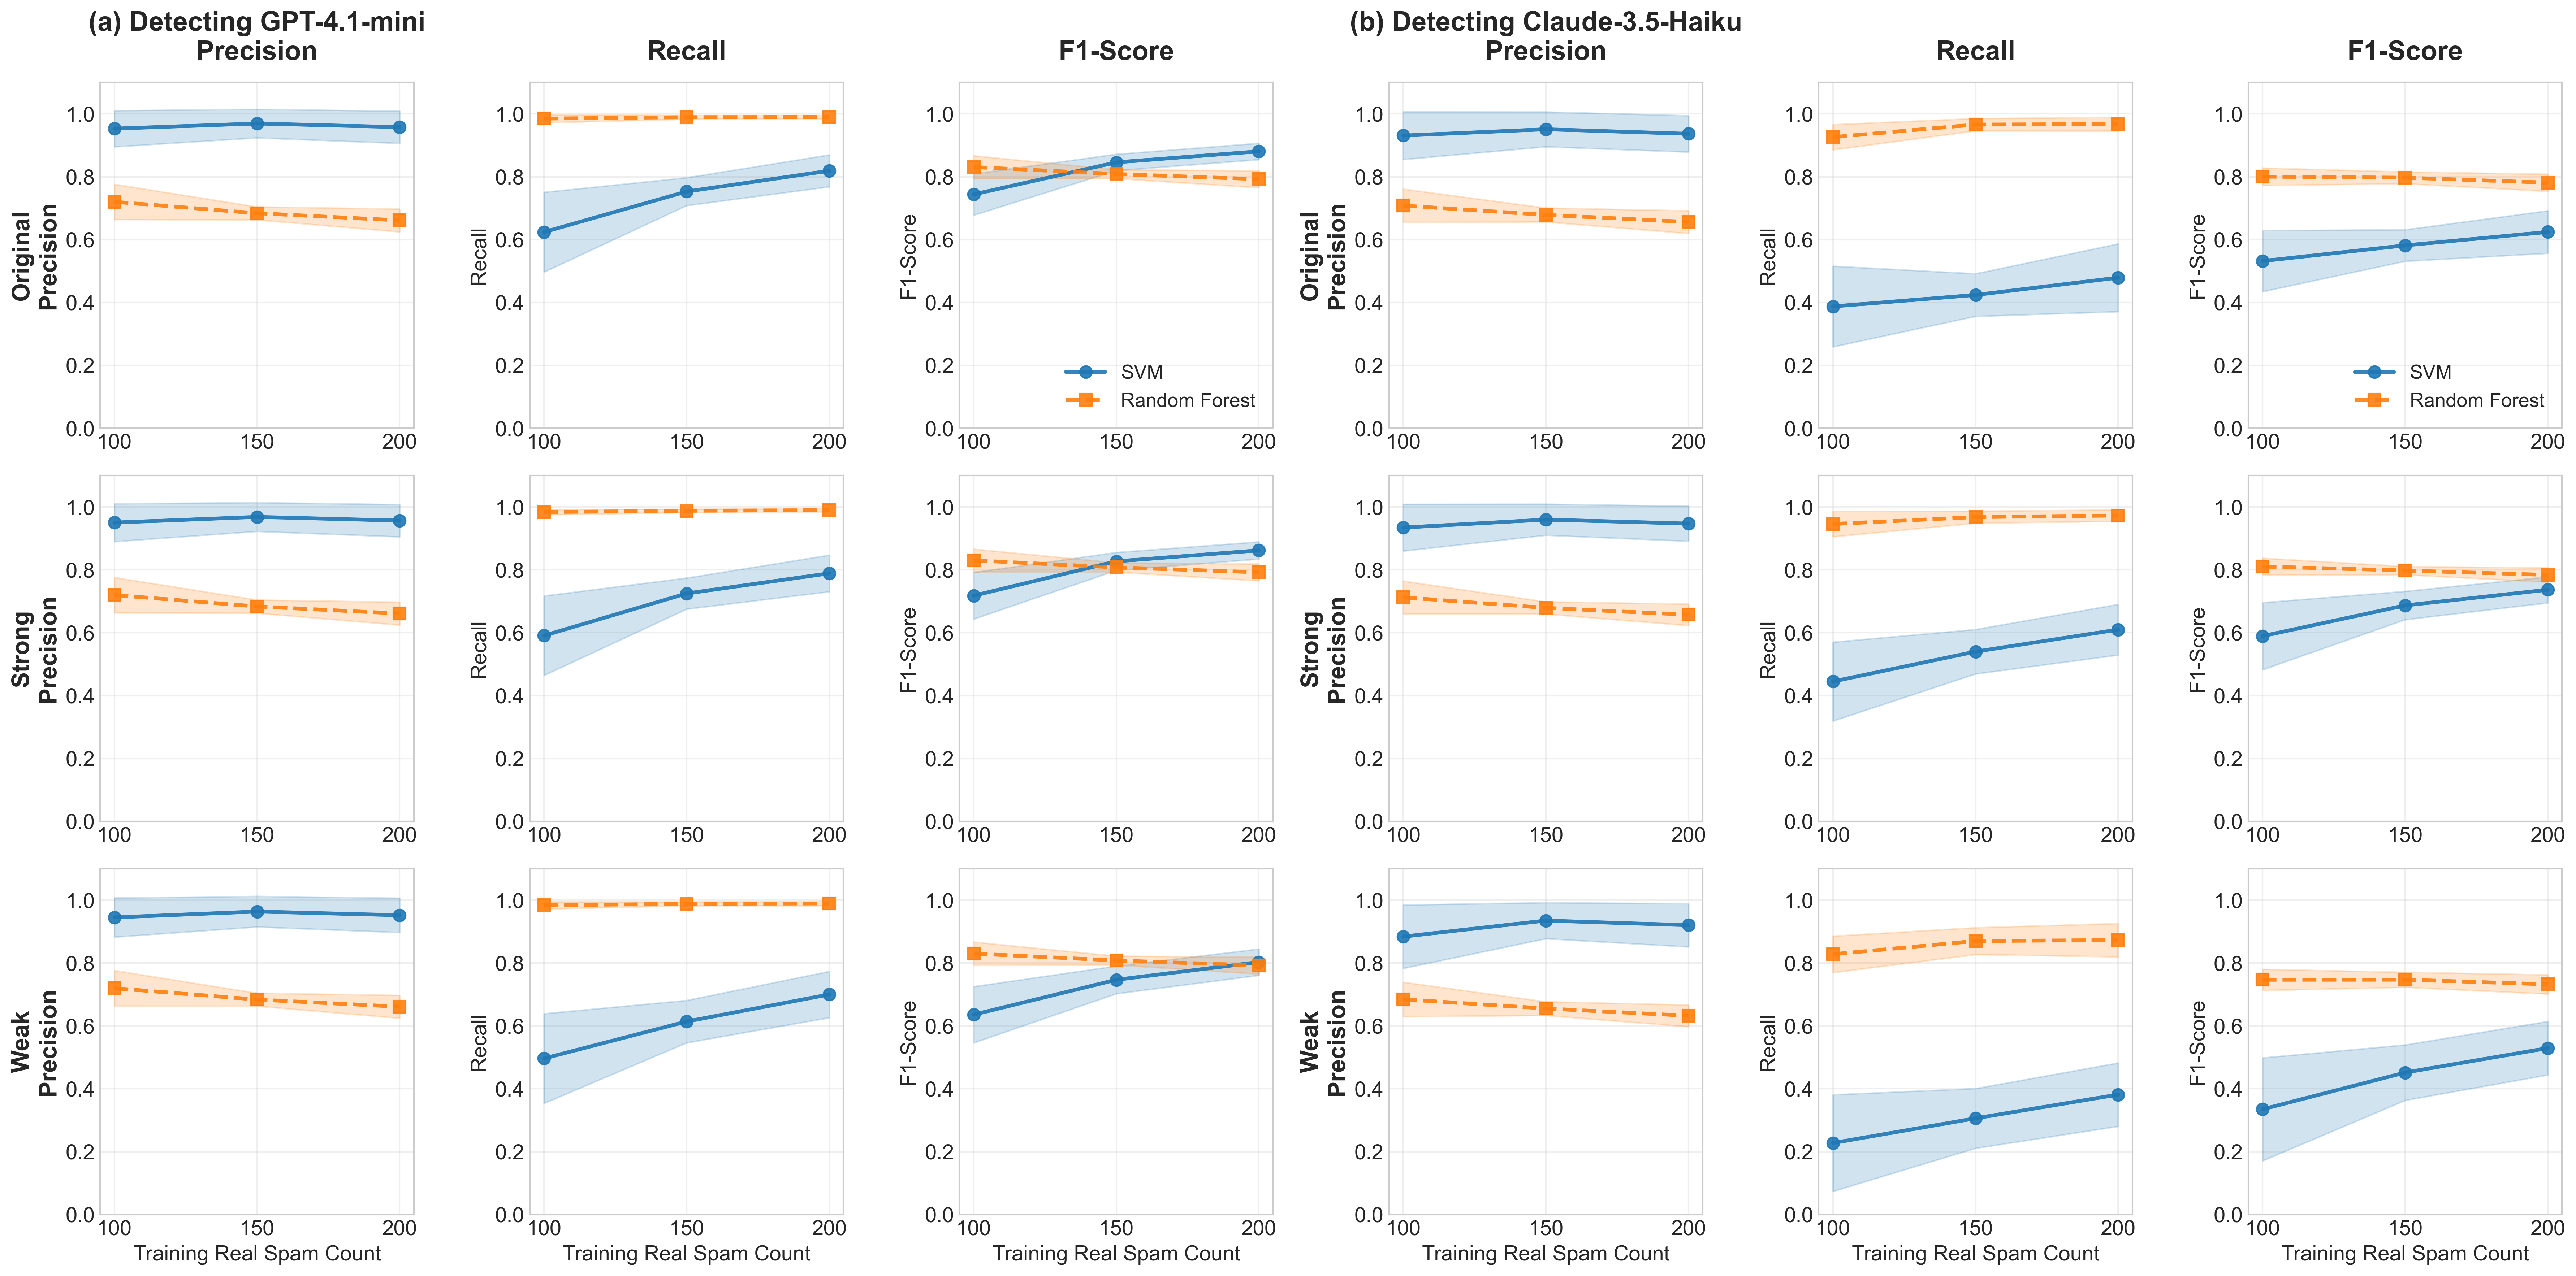
\includegraphics[width=\textwidth]{pic/track2a_combined_gpt_claude.png}
\caption{Track 2a - Real-to-Synthetic Detection: Performance metrics (Precision, Recall, F1-Score) across prompt strategies (rows) and models (columns). (a) Detecting GPT spam: SVM F1 = 0.74-0.82, RF F1 = 0.82-0.87, with SVM showing increasing F1 as training data grows while RF remains stable. (b) Detecting Claude spam: SVM shows moderate detection improving with more training data (F1 = 0.53-0.74 across prompts), while RF maintains strong performance (F1 = 0.80-0.85).}
\label{fig:track2a}
\end{figure*}



\begin{table*}[t]
\centering
\caption{Track 2a \& 2b: Real-to-Synthetic and Mixed-to-Synthetic Detection Performance}
\label{tab:track2a_2b_combined}
\resizebox{\textwidth}{!}{
\begin{tabular}{lllcccccc}
\toprule
\textbf{Testing} & \textbf{Prompt} & \textbf{Classifier} & \multicolumn{3}{c}{\textbf{Track 2a: Real-to-Synthetic}} & \multicolumn{3}{c}{\textbf{Track 2b: Mixed-to-Synthetic}} \\
\cmidrule(lr){4-6} \cmidrule(lr){7-9}
\textbf{Target} & & & \textbf{100} & \textbf{150} & \textbf{200} & \textbf{0\%} & \textbf{50\%} & \textbf{100\%} \\
\midrule
\multirow{6}{*}{GPT-4.1-mini} & \multirow{2}{*}{Original} & SVM & 0.744 $\pm$ 0.064 & 0.846 $\pm$ 0.025 & 0.881 $\pm$ 0.025 & 0.744 $\pm$ 0.064 & 0.770 $\pm$ 0.035 & 0.649 $\pm$ 0.042 \\
 & & Random Forest & 0.831 $\pm$ 0.035 & 0.809 $\pm$ 0.014 & 0.792 $\pm$ 0.026 & 0.824 $\pm$ 0.025 & 0.816 $\pm$ 0.023 & 0.894 $\pm$ 0.030 \\
 & \multirow{2}{*}{Strong} & SVM & 0.718 $\pm$ 0.072 & 0.827 $\pm$ 0.028 & 0.862 $\pm$ 0.027 & 0.718 $\pm$ 0.072 & 0.822 $\pm$ 0.040 & 0.696 $\pm$ 0.110 \\
 & & Random Forest & 0.830 $\pm$ 0.035 & 0.808 $\pm$ 0.014 & 0.792 $\pm$ 0.026 & 0.824 $\pm$ 0.026 & 0.827 $\pm$ 0.032 & 0.908 $\pm$ 0.040 \\
 & \multirow{2}{*}{Weak} & SVM & 0.636 $\pm$ 0.087 & 0.747 $\pm$ 0.043 & 0.803 $\pm$ 0.041 & 0.636 $\pm$ 0.086 & 0.822 $\pm$ 0.038 & 0.688 $\pm$ 0.119 \\
 & & Random Forest & 0.830 $\pm$ 0.036 & 0.808 $\pm$ 0.014 & 0.792 $\pm$ 0.026 & 0.824 $\pm$ 0.028 & 0.822 $\pm$ 0.026 & 0.834 $\pm$ 0.061 \\
\midrule
\multirow{6}{*}{Claude-3.5-haiku} & \multirow{2}{*}{Original} & SVM & 0.532 $\pm$ 0.095 & 0.582 $\pm$ 0.049 & 0.624 $\pm$ 0.066 & 0.532 $\pm$ 0.094 & 0.666 $\pm$ 0.031 & 0.688 $\pm$ 0.033 \\
 & & Random Forest & 0.800 $\pm$ 0.027 & 0.797 $\pm$ 0.018 & 0.781 $\pm$ 0.026 & 0.802 $\pm$ 0.021 & 0.802 $\pm$ 0.020 & 0.802 $\pm$ 0.022 \\
 & \multirow{2}{*}{Strong} & SVM & 0.589 $\pm$ 0.104 & 0.687 $\pm$ 0.044 & 0.737 $\pm$ 0.040 & 0.590 $\pm$ 0.104 & 0.827 $\pm$ 0.032 & 0.860 $\pm$ 0.033 \\
 & & Random Forest & 0.811 $\pm$ 0.026 & 0.798 $\pm$ 0.013 & 0.784 $\pm$ 0.022 & 0.806 $\pm$ 0.023 & 0.814 $\pm$ 0.024 & 0.823 $\pm$ 0.027 \\
 & \multirow{2}{*}{Weak} & SVM & 0.335 $\pm$ 0.160 & 0.452 $\pm$ 0.086 & 0.529 $\pm$ 0.083 & 0.335 $\pm$ 0.160 & 0.748 $\pm$ 0.038 & 0.805 $\pm$ 0.026 \\
 & & Random Forest & 0.747 $\pm$ 0.033 & 0.747 $\pm$ 0.023 & 0.732 $\pm$ 0.030 & 0.748 $\pm$ 0.031 & 0.777 $\pm$ 0.032 & 0.813 $\pm$ 0.021 \\
\bottomrule
\end{tabular}
}
\end{table*}

Classifier architecture determines sensitivity to training data quantity for zero-shot detection. SVM exhibits substantial monotonic improvement with additional real spam (for GPT detection: F1 from 0.744 at 100 samples to 0.881 at 200 samples), while Random Forest (RF) maintains stable performance across training sizes (F1 $\approx$ 0.83 for GPT, $\approx$ 0.80 for Claude). This divergent behavior reflects fundamental architectural differences: margin-based learning requires more training examples to accurately position decision boundaries, while ensemble aggregation achieves near-optimal feature learning at minimal training size.

Detection difficulty varies by model and prompt strategy. For GPT synthetic spam, SVM achieves highest performance on original prompts (F1 = 0.744 at 100 samples), while RF shows near-perfect prompt invariance (F1 $\approx$ 0.83). For Claude synthetic spam, the pattern reverses with strong prompts yielding highest detectability. Weak prompts universally yield lowest detection across both models (Claude weak: SVM F1 = 0.335), creating spam that confounds classifiers trained on real data through distributional divergence. These findings establish that prompt optimization for evasiveness differs by LLM source.

Model-dependent baseline detectability reveals generation quality differences. At 100 training samples, GPT synthetic spam exhibits higher detectability (SVM: 0.636-0.744, RF: 0.830-0.831) compared to Claude synthetic spam (SVM: 0.335-0.589, RF: 0.747-0.811). This higher detectability paradoxically correlates with GPT's superior performance in Track 1, suggesting distributional proximity to real spam enables both effective classifier training and effective detection.

% Random Forest demonstrates superior prompt invariance, maintaining remarkably consistent performance across all prompt strategies while SVM shows substantial variance. This robustness indicates ensemble methods effectively extract prompt-invariant features for AI-spam detection, providing more reliable defense against varied generation strategies.

\subsection{Track 2b: Mixed-to-Synthetic Detection}
\label{sec:eval:track2b}

% Figure~\ref{fig:track2b} presents detection performance metrics (Precision, Recall, F1-Score) across varying synthetic training ratios and prompt strategies. Table~\ref{tab:track2a_2b_combined} (Track 2b columns) presents enhanced detection performance across all experimental configurations, demonstrating how training with synthetic spam from one LLM affects detection of synthetic spam from a different LLM.

% Figure~\ref{fig:track2b} and Table~\ref{tab:track2a_2b_combined} (Track 2b columns)

\begin{figure*}[t]
\centering

\includegraphics[width=\textwidth]{pic/track2b_combined_gpt_claude.png}
\caption{Track 2b - Mixed-to-Synthetic Detection: Performance metrics (Precision, Recall, F1-Score) across prompt strategies (original/strong/weak, rows) and detection targets (columns). (a) Detecting GPT (trained on Claude synthetic): SVM peaks at 50\% synthetic (F1 = 0.77, +3.5\%) before declining at 100\% (F1 = 0.65, -13\%). RF improves substantially with cross-model augmentation (F1: 0.82 $\rightarrow$ 0.89, +8.5\%). (b) Detecting Claude (trained on GPT synthetic): SVM shows monotonic improvement (F1: 0.53 $\rightarrow$ 0.69, +30\% relative). RF maintains stable high performance (F1 $\approx$ 0.80) across all ratios.}
\label{fig:track2b}
\end{figure*}




Cross-model synthetic augmentation provides substantial but variable detection improvements depending on baseline performance. Training with synthetic spam from one LLM significantly improves detection of another LLM's synthetic spam, with gains ranging from moderate to dramatic. For Claude detection using GPT synthetic training data, SVM achieves substantial improvements at 100\% synthetic (strong prompt: F1 from 0.590 to 0.860, +45.8\% relative). For GPT detection using Claude synthetic training data, RF achieves +8.5\% improvement (F1: 0.824 $\rightarrow$ 0.894 for original prompt). These findings indicate cross-model augmentation provides measurable benefits across configurations, though absolute gains matter more than relative percentages when baselines differ substantially.

Prompt-dependent augmentation effectiveness reveals generation diversity impact. For Claude detection, weak prompt training data achieves F1 = 0.805 compared to original prompt training (F1 = 0.688), suggesting diverse, lower-quality synthetic spam better captures the full feature space of AI-generated content. This counterintuitive pattern indicates training on varied generation characteristics enables more robust detection across generation strategies than training exclusively on high-quality synthetic samples.

Random Forest exhibits remarkable cross-model robustness with prompt-invariant detection. For both GPT and Claude detection, RF maintains stable baseline performance across prompts (F1 $\approx$ 0.75-0.83) and achieves consistent improvements with synthetic augmentation. In contrast, SVM exhibits substantial baseline variance across prompts (F1 range: 0.335-0.744) and less consistent augmentation benefits. This indicates ensemble methods effectively extract cross-model and cross-prompt invariant features, providing reliable detection across diverse generation conditions.

Optimal synthetic ratios exhibit complex dependencies on target model and classifier architecture. For Claude detection using GPT synthetic training data, most configurations show monotonic improvement with increasing synthetic ratio. For GPT detection using Claude synthetic training data, patterns diverge by classifier: RF consistently benefits from high synthetic ratios (optimal at 100\%, F1 = 0.834-0.908), while SVM demonstrates non-monotonic behavior with peak performance at 50\% (F1 = 0.770-0.822) before declining at 100\% (F1 = 0.649-0.696). This SVM degradation suggests overfitting to distributional artifacts when training exclusively on cross-model synthetic spam, while Random Forest's ensemble mechanism provides inherent regularization.